\chapter{Implementasi dan Pengujian}

\section{Implementasi}

\subsection{Lingkungan Implementasi}

Sistem implementasi dan fungsi kosakata dikembangkan dan diuji pada lingkungan yang sama, yaitu lingkungan lokal dalam sebuah gawai laptop. Berikut adalah spesifikasi lingkungan yang digunakan:

\begin{enumerate}
    \item Spesifikasi Perangkat Keras:
    \begin{enumerate}
        \item Perangkat \tab : ASUS X450LD tahun 2014
        \item Prosessor \tab : 1,6 GHz Intel Core i5 4200U
        \item Memori \tab : 4 GB DDR3
        \item Penyimpanan \tab : HDD 500 GB
        \item Sistem Operasi \tab : Windows 10 64bit
    \end{enumerate}
    \item Alat Pengembangan: Visual Studio Code, Anaconda, Jupyter Notebook
    \item Bahasa Pemrograman: Python 3.6.5 64bit
    \item \textit{Library} yang Digunakan: NLTK, Keras, Numpy
\end{enumerate}

\subsection{Sistem Implementasi}

Untuk dapat mengimplementasikan fungsi kosakata, diperlukan sebuah sistem yang mendukung keberjalanan fungsi tersebut.

\subsection{Implementasi Fungsi Kosakata}

Fungsi kosakata yang telah dibangun diimplementasi

Implementasi dari fungsi kosakata diterapkan dalam sistem klasifikasi kalimat. Gambar \ref{fig:design_classification} adalah diagram alur proses dari sistem klasifikasi kalimat, dengan penjelasan tiap proses adalah sebagai berikut:

\begin{enumerate}
	\item sistem menerima masukan teks dari \textit{speech recognition} yang dimasukkan oleh suara pengguna,
	\item sistem memecahkan teks menjadi sekumpulan \textit{token},
	\item sistem mengenali entitas yang berada di dalam teks, kemudian mengekstraksi entitas tersebut,
	\item sistem menciptakan tas kata-kata untuk teks masukan,
	\item sistem melakukan prediksi maksud kalimat dari masukan tas kata-kata menggunakan model klasifikasi yang dihasilkan pada tahap latihan klasifikasi,
	\item maksud kalimat yang telah dihasilkan, bersama dengan kumpulan entitas hasil ekstrasi, dikumpulkan lalu diubah kedalam format JSON, dan,
	\item JSON dikirimkan kepada pengguna.
\end{enumerate}

\begin{figure}[H]
	\centering
	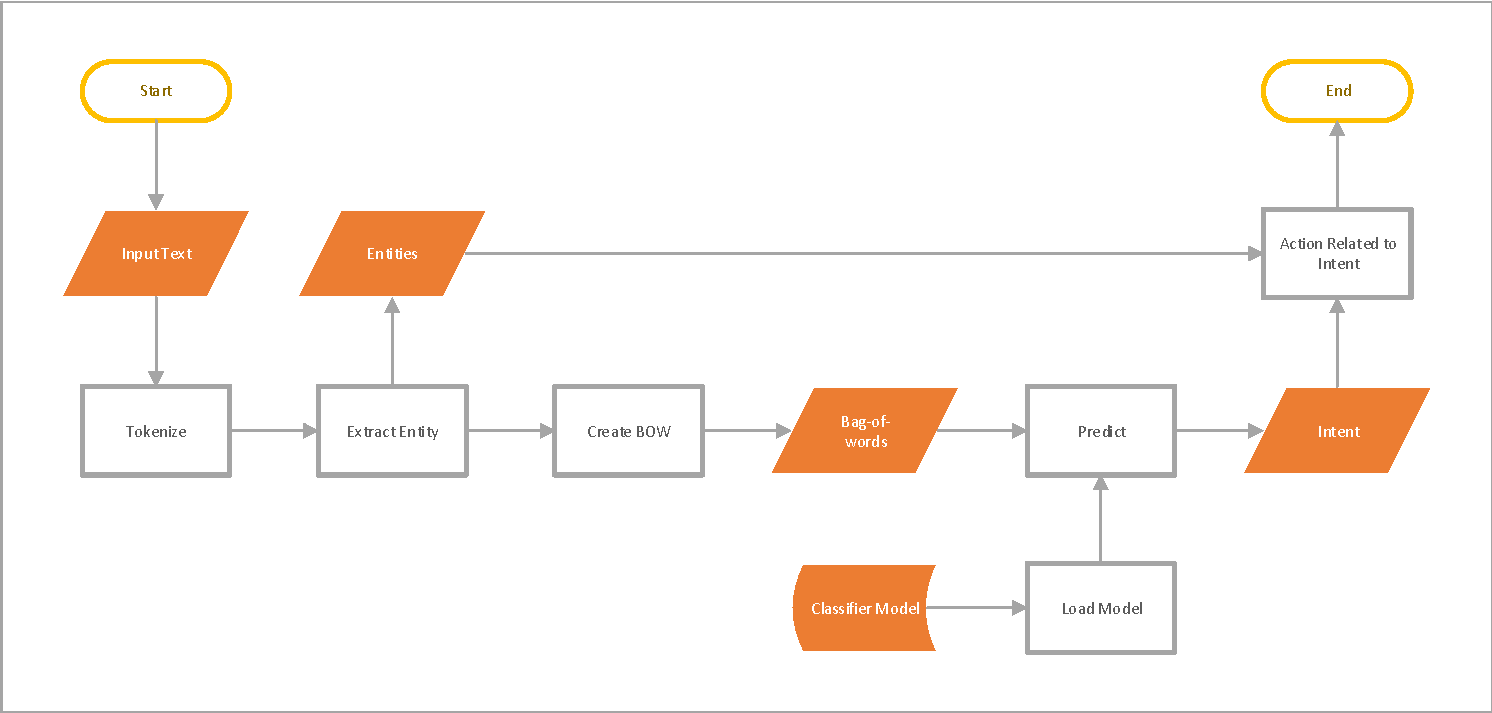
\includegraphics[width=\textwidth, trim=2 2 2 2, clip]{resources/4/design_classification.pdf}
	\caption{Bagan rancangan sistem tahap klasifikasi teks}
	\label{fig:design_classification}
\end{figure}

Proses yang akan diterapkan fungsi kosakata adalah proses pengenalan entitas. Kalimat yang entitasnya akan dikenali, terleih dahulu harus diubah menjadi sekumpulan indeks. Indeks tersebut mengacu kepada kosakata yang telah didefinisikan pada sistem latihan klasifikasi kalimat.

\section{Pengujian}

\subsection{Lingkungan Pengujian}

Pengujian untuk kedua sistem SLU bagian pelatihan, Rasa NLU dan sistem baru, yang akan diukur dan dibandingkan kemampuannya, dilakukan dengan menggunakan komputer lokal. Spesifikasi lingkungan untuk komputer adalah sebagai berikut:

\begin{enumerate}
    \item Windows 10,
    \item Python 3.6 dari Anaconda,
    \item \textit{Library} Keras, dan,
    \item \textit{Library} scikit-learn.
\end{enumerate}

Sebelum melakukan pengujian, kedua sistem terlebih dahulu melakukan pelatihan pada sebuah \textit{file} JSON yang disiapkan sebagai data latih. \textit{File} JSON tersebut berisi kumpulan kalimat-kalimat perintah berbentuk teks, beserta dengan maksud kalimat tersebut dan entitas-entitas yang terkandung di dalamnya.

Pengujian dilakukan dengan memasukkan data pengujian dari survey kepada beberapa orang. Masukan tersebut diubah terlebih dahulu menjadi format JSON. Lalu, kedua sistem harus melakukan prediksi dari data pengujian yang telah diberikan. Kemudian, hasil prediksi tersebut dievaluasi menggunakan skrip Perl untuk evaluasi CoNLL tahun 2000 \parencite{tjong2000introduction}.

Parameter yang digunakan untuk hasil pengujian adalah \textit{precision}, \textit{F1-score}, dan \textit{recall}.

\subsection{Hasil Pengujian}

Tabel \ref{tbl:result} menunjukkan hasil dari pengujian kedua sistem.

\begin{table}[H]
    \caption{Hasil Pengujian}
    \label{tbl:result}
    \centering
    \begin{tabular}{|l|c|c|c|}
        \hline
                                                       & \textit{\textbf{Precision}} & \textit{\textbf{F1}} & \textit{\textbf{Recall}} \\ \hline
        \textit{\textbf{Conditional Random Field}}     & 17.07                       & 29.17                & 21.54                    \\ \hline
        \textit{\textbf{Convolutional Neural Network}} & 31.71                       & 35.14                & 33.33                    \\ \hline
    \end{tabular}
\end{table}